\documentclass[twocolumn]{article}
\usepackage{fullpage}
\usepackage{amssymb}
\usepackage{fancyvrb}
\usepackage{url}
\usepackage{proof}
\usepackage{code}
\usepackage{graphicx}

\begin{document}

\newcommand\currentrevision{532}
\newcommand\currentsizekb{250}
\newcommand\wikipliaurl{http://wikiplia.spacebar.org/}

\newcommand\ftinker{\ensuremath{\copyright}}
\newcommand\fexpression{\ensuremath{\hbar}}
\newcommand\fbeer{\ensuremath{\triangle}}
\newcommand\fusa{\ensuremath{\sqrt[x^{1.2}]{\mbox{\t{oo}} + \frac{x}{z^2}}}}
\newcommand\ffree{\ensuremath{\P}}
\newcommand\ftobe{{\tiny \ensuremath{\stackrel{\bigcirc}{\amalg}}}}

\newcommand\wcite[1]{\footnote{\tiny Wikipedia, the free encyclopedia: {\it #1}; 2007}}
\newcommand\wciteshort[1]{\footnote{\tiny Wikipedia, the free encyclopedia: {\it #1}}}
\newcommand\comment[1]{}
\newcommand\z{\ensuremath{\!}}

\newcommand\D\Delta
\newcommand\G\Gamma
\newcommand\m\mapsto
\newcommand\eval{{\sf eval\,\,}}
\newcommand\tag[2]{{\tt{\mbox{\tt <}}{#1}{\mbox{\tt>}}}{#2}{\tt{\mbox{\tt</}}{#1}{\mbox{\tt>}}}}
\newcommand\prim{{\,\,\sf prim}}
\newcommand\rate{{\sf rate\,\,}}

\newcommand\lb{\ensuremath{[\![}}
\newcommand\rb{\ensuremath{]\!]}}

\title{{\bf \huge Wikiplia}:\\
       The Free Programming Language\\
       That Anyone Can Edit}

\author{Tom Murphy VII}
\date{1 April 2007}

\maketitle

\begin{abstract}
We present a new programming language called Wikiplia. The language
has an unprecedented level of integration: The system is its own
compiler, language definition, documentation, development environment,
distributed filesystem, database, revision control system,
bootstrapping software license, community message board, and World
Wide Web home site. Wikiplia is designed to be Free to a greater
extent and in more dimensions than existing languages.
\end{abstract}

\footnotetext[-1]{Copyright \copyright\ 2007 the Regents of the Wikiplia
Foundation. Appears in SIGBOVIK 2007 with the permission of the
Association for Computational Heresy; {\em IEEEEEE!} press,
Verlag-Verlag volume no.~0x40-2A. This document may be distributed
under the terms of the TIA Public License (Section~\ref{sec:license}).
\pounds 0.00}

\vspace{1em}
{\noindent \small {\bf Keywords}:
  Freedom, programming language, software license, wiki, XML, 
  weatherproof footwear and their fastening mechanisms,
  hyper-driven devices
}

\section{Introduction}

One of the most cherished social principles of mankind is
freedom,\z\wcite{Freedom} in its many incarnations. More recently,
freedom has become an important principle in computer science as well,
with the introduction of Free Software licenses such as the GNU
GPL,\z\wcite{GNU General Public License} extensible markup languages
such as XML,\z\wcite{XML} the ability explicitly deallocate memory
with the {\tt free(3)} library call, and the widespread availability of
Free Herbal V1agara on the World Wide Web.\z\wcite{Sildenafil}

The aim of this project is to develop a programming language that is
as free as possible. We begin by enumerating freedoms that we desire
to support. Because freedom is a possession of inestimable
value\wcite{Cicero} we do not attempt to rank these freedoms; instead,
each freedom is ``numbered'' using a symbol drawn from incomparable
sets of glyphs.

\paragraph{Freedom \ftinker: The freedom to tinker.}
Users should be able to study a program to see how it works, and to
make modifications to suit his or her needs. For most software, this
means that the programmer needs access to the software's
documentation, source code, and UML\wcite{Unified Modeling Language}
use case diagrams. This is traditionally achieved through licenses
such as the GPL; however, as we will discuss in
Section~\ref{sec:bootstrap} there are special considerations for
bootstrapping compilers that render the GPL inadequate for this
purpose.

\paragraph{Freedom \fexpression: Freedom of expression.}
Programmers should be able to write their programs using any
expressions that they like. Specifically, there should be no
prior establishment of arbitrary categories of expression that
are excluded, such as those that discriminate on the basis
of class, mathematical philosophy, or type.

\paragraph{Freedom \ftobe: Free to be You and Me.}
The development of a programming language should not be confined to
the bearded academic elite, gazing down upon the programmer fiefs from
their stratospheric ivory towers. Wikiplia is the free programming
language that {\em anyone} can edit: from bearded academic
elite\wcite{Tenure} to congressional staffers\wciteshort{Congressional
staffer edits to Wikipedia} to nameless Slashdot\wcite{Slashdot}
trolls. Wikiplia's WWW-based approach means that an Internet
connection and compatible WWW hypertext browser is all that's needed
to begin on the life-changing journey of programming language design.

% freedom of speech?

\paragraph{Freedom \fbeer: Freedom of beer.}
Users should be able to write software without paying money to a
licensing authority or certification program.

\paragraph{Freedom \ffree: Freedom to redefine freedom.}
Freedom should be free, so the definition of freedom should be free to
change as the meaning of freedom changes. Wikiplia's license allows
for Wikiplia to be distributed in a way that monotonically increases
freedom as new concepts and catchphrases of freedom are invented.

\paragraph{Freedom \fusa: Freedom of USA \#1.}
Wikiplia is 100\% made in the USA and only available in
English.\z\wcite{Freedom fries}

% XXX more...

\section{Reflections on strapping straps and booting boots} \label{sec:bootstrap}

The hallmark of Free software is the GNU General Public License. It is
a hereditary license that requires that (a) source code be distributed
with the program and (b) modified versions of the program also be
licensed under the GPL. The intention is that anyone receiving the
software can exercise Freedom~\ftinker\ by understanding the source
code and modifying it to suit his needs. Clearly any source code will
not do: an obfuscated\wcite{Obfuscated code} version of the source
code cannot be easily understood or modified, even though it is
technically ``source code.'' The GPL therefore legally defines source
code as the ``preferred form'' for ``making modifications.''

Even source code in the preferred form might not be enough to achieve
Freedom~\ftinker, however. For instance, the program might be written
in a mysterious programming language that only the author understands,
and that programming language might only be implemented in a private
compiler on the author's hard disk.\z\wcite{Hard disk} It is therefore
reasonable to construe the ``preferred form'' of the original software
to include the implementation of the programming language that the
software is written in. Because the programmer might need to fix bugs
or extend the programming language implementation in order to modify
the original program, he also needs the source code for that language
as well. This code must also be written in some language, so the
process continues. It can end when one of the programming languages is
generally well known enough that there are no practical barriers to
understanding it or finding an implementation (examples would include
C\wcite{C (programming language)} and ALGOL 58\wcite{ALGOL 58}), or so
simple that the implementation is essentially non-existent ({\em e.g.}
an assembler implemented directly in machine code).

Another way for this process to terminate is for a programming
language to be implemented in itself. This is known as a
``bootstrapping compiler.'' A natural social tendency causes this to
be very common: language implementors are more likely to enjoy the
language they are implementing, and therefore more likely to choose it
to implement the language. But when this process terminates this way,
the reader might be left with a suspicious sense that nothing has
actually been achieved.\z\footnote{In the case of a LOGO interpreter
implemented in LOGO, we could say that this is then ``turtles all the
way down.''} Specifically: What freedom-fulfilling use is the source
code to an implementation of a mysterious programming language, if
that source code is itself in the same mysterious programming
language?

Let us concentrate on a more concrete example. The GNU C
compiler\wcite{GNU Compiler Collection} (licensed under the GPL) is
an implementation of the C language with some extensions specific to
the compiler. The GCC source code uses some of these extensions. Can
the GCC be Free software if it requires the GCC to build? In the
extreme case, what if someone were to add an extension to the GCC to
enable a new C keyword---called {\tt compile\_a\_program}---and then
replace the entire source code with:

\begin{code}
int main (int argc, char ** argv) \{
  compile_a_program;
  return 0;
\}
\end{code}

Such code is clearly worthless. Not all subversions of the source code
via language extension may be so overt, but we claim that they
nonetheless pose a substantial threat to freedom.

We do not wish to limit the programmer's ability to make extensions to
a language, since this would also toe-step Freedom~\ftinker. We then
conclude that the licensing terms must be expanded in order to provide
more than ``source code.'' We propose that not only the source, but
the source code's {\em history}, must be made available.

\subsection{Revision control}

Computer scientists use revision control\wcite{Revision control} to
track changes to software and to coordinate development between
multiple programmers. This has been true for thousands of years.
Popular revision control systems such as CVS\wcite{Concurrent Versions
System} and Subversion\wcite{Subversion (software)} allow for code
to be concurrently modified by two or more developers and then have
their changes integrated after the fact by an explicit ``check in''
and conflict resolution phase.

It may na\"\i{}vely seem that publishing the entire CVS history of a
project would solve the issue with language extensions: By inspecting
the revision that introduced the {\tt compile\_a\_program} feature
(but prior to the replacement of the GCC with the minuscule version
above), one could then see its implementation and then know what it
means. For certain patterns of development this does indeed suffice.
However, programmers are not forced to check in their changes except
at their own whims, as determined by social conventions; a programmer
might make the private addition of the keyword {\tt
compile\_a\_program}, then rewrite the GCC to use it, and only then
check in this change as one revision. For this action he will surely
be rebuked by his fellow programmers; none of the other developers can
compile the new version of the code without access to the intermediate
revision! This social pressure would also na\"\i{}vely seem to be enough
to address the problem, but more insidious scenarios yet obtain.

As a concrete example, suppose there are two programmers called K and
R. Each is modifying the GCC with the purpose of adding a new
character constant, \verb+'\c'+. K and R start at revision 100 of the
GCC. K finds the case analysis for parsing character constants:
%
\begin{code}
/* REVISION 100 (K) */
switch(ch) \{
  case 'n': return '\\n';
  case 'r': return '\\r';
  \vdots
  default: abort("bad char constant");
\}
\end{code}
%
He adds a case for his extension, without using the extension, and
checks this in as revision 101.
%
\begin{code}
/* REVISION 101 (K) */
switch(ch) \{
  case 'n': return '\\n';
  case 'r': return '\\r';
  \vdots
  case 'c': return 257;
  default: abort("bad char constant");
\}
\end{code}
%
Meanwhile, R has similar (but not identical) inspiration and modifies
his copy of the compiler:
%
\begin{code}
/* REVISION 100 (R) */
switch(ch) \{
  case 'n': return '\\n';
  case 'r': return '\\r';
  \vdots
  case 'c': return 8675309;
  default: abort("bad char constant");
\}
\end{code}
%
He does not commit his code because he is wary of the time-consuming
conflict resolution phase and is late for a date with K's estranged
wife who is fed up with K's all-night hacking binges. He burns rubber
in his 2007 Honda Civic\wcite{Honda Civic} with aftermarket spoiler
for a night on the town, believing that a healthy well-rounded
programmer spends more or less equal nights basking in the pale amber
glow of the teletype as waking up with a few missing teeth naked and
norovirused in some midtown alleyway with his wallet barely out of
reach but empty anyway, having amply exercised Freedom~\fbeer.

Meanwhile, K continues extending the GCC, using the extension to
implement itself. He checks in this code with no conflicts:
%
\begin{code}
/* REVISION 102 (K) */
switch(ch) \{
  case 'n': return '\\n';
  case 'r': return '\\r';
  \vdots
  case 'c': return '\\c';
  default: abort("bad char constant");
\}
\end{code}
%
K punches out at {\tt 1130 UTC},\z\wcite{Coordinated Universal Time}
just as R returns from his adventure. R's confidence bolstered, he
finishes his extension effort, following best practices and
implementing the extension using itself:
%
\begin{code}
/* REVISION 100 (R) */
switch(ch) \{
  case 'n': return '\\n';
  case 'r': return '\\r';
  \vdots
  case 'c': return '\\c';
  default: abort("bad char constant");
\}
\end{code}
%
He now decides to commit his changes (forgetting that he did not
commit the intermediate revision). To do so he updates to the newest
revision, 102, and sees that there are no conflicts---in fact,
revision 102 already contains his changes! Believing that his changes
are therefore compatible, he continues hacking.

After this scenario, K and R believe they are working on the same
programming language---after all, it has the same source code---but
their minor bifurcation in development history means that they have
forever different meanings of the \verb+'\c'+ extension. This mistake
is likely to go unnoticed for some time, and until it is resolved, the
meaning of the \verb+'\c'+ extension is firmly enslaved in the
bipartite penitentiary of double entendre, yearning to be
free\,\ldots\z\wcite{Information wants to be free}

\subsection{Solution}

Based on these scenarios we conclude that extant social measures such
as revision control conventions are not enough to guarantee freedom.
Even if we think these situations are implausible in the hands of
well-intentioned, well-mannered and capable%
%
\wcite{Year 2000 problem}$^,$%
\wciteshort{Northeast Blackout of 2003}$^,$%
\wcite{Ariane 5 Flight 501}$^,$%
\wcite{Mars Climate Orbiter}$^,$%
\wcite{Mars Polar Lander}$^,$%
\wcite{Mars Rover}$^,$%
\wcite{Mars Pathfinder}$^,$%
\wcite{Gripen\#Crashes}$^,$%
\wcite{missingno.}$^,$%
\wcite{XSS}$^,$%
\wcite{Buffer overflow}$^,$%
\wcite{Therac-25}$^,$%
\wcite{Lothar (storm)}$^,$%
\wcite{Mariner 1}$^,$%
\wcite{Code Red worm}$^,$%
\wcite{SQLSlammer}$^,$%
\wcite{Sandstorm (vehicle)}$^,$%
\wcite{Samy (XSS)}$^,$%
\wcite{Pentium FDIV bug}$^,$%
\wcite{MIM-103 Patriot}$^,$%
\wcite{Windows 95}$^,$%
\wcite{Morris (computer worm)}$^,$%
\wcite{USS Yorktown (CG-48)}
%
software engineers, we wish for our software to remain free even when
in the hands of nefarious and crafty factions who would seek to
fracture\wcite{Fork (software development)} our free software
community. We therefore need a technological and legal solution that
forces the entire development history to be available. Keeping with
Freedom~\fusa, we call this technology and its license {\em Total
Information Awareness} after the successful project of the US
Government with the same name.\z\wcite{Information Awareness Office}

Technologically, we develop our system around a primitive notion of
revision control in which every change to the system is recorded.
Because the system has an integrated editor, every action of a
programmer is logged and preserved indefinitely with no extra action
necessary on the programmer's part. Such commits are globally atomic,
using a single universal repository. (This means that in the above
scenario, R would not have been able to forget to commit his
intermediate change, and would have been forced to observe his
conflict with K.) To protect against the possibility that divergent
development paths lead to incompatible compilers, we require that
there is only one compiler for any given programming language, which
itself exists in the revision control system. Therefore, it is always
clear which version of the compiler was used to produce an executable
from source. This also makes the K and R scenario impossible: there is
only one compiler and so it is impossible for it to differ from
itself.

Legally, all of the software is licensed (Section~\ref{sec:license})
under terms similar to the GNU GPL, but that define the ``source
code'' to include the entire revision history of the system. In order
to be compatible with Freedom~\ffree, we allow the license itself to be
edited, but to ensure that no one can remove freedoms already present
in the license, the license includes a provision that allows any {\em
prior} version of the license to be used, at the programmer's option.

\subsection{Implementation}

Wikiplia, the free programming language that anyone can edit, is
implemented as a web-site on the Internet at the address
$${\tt \wikipliaurl}$$

\subsection{Roadmap}

The remainder of this paper proceeds as follows. We first present in
Section~\ref{sec:calculus} the design of the initial Wikiplia system,
which is used to bootstrap the rest of Wikiplia. We then discuss the
current state of Wikiplia as of revision \currentrevision\ in
Section~\ref{sec:current}. We explain the freedom-preserving TIA
Public License in Section~\ref{sec:license}. We conclude with a
discussion of unrelated work and plans for the future~\ref{sec:conc}.

\section{Core calculus} \label{sec:calculus}

\begin{figure}[ht]

\comment{
    List of exp list       <list> ... </list>
  | String of string       <string>s</string>
  | Int of IntInf.int      <int>i</int>
  | Symbol of string       <symbol>s</symbol>
  (* the only lazy expression *)
  | Quote of exp           <quote>exp</quote>
  (* user can't write these *)
  | Prim of prim           <prim>p</prim>
  | Closure of (string * exp) list * string * exp
}
\begin{center}
\begin{tabular}{rcl}
 {\em X} & ::= & {\tt<}{\em tag}{\tt >} $X_1\ X_2\ \ldots\ X_n$ {\tt</}{\em tag}{\tt >} \\
         & $|$ & string
\end{tabular}
\end{center}
\caption{Syntax of XML} \label{fig:xml}
\end{figure}

\begin{figure*}[ht]
\[\begin{array}{cc}
% basic, easy
\infer{\G \vdash \eval \tag{string}{s} \m \tag{string}{s}}{} &
\infer{\G \vdash \eval \tag{quote}{X} \m X}{} \\[1em]
\infer{\G \vdash \eval \tag{int}{s} \m \tag{int}{s}}{} &
\infer{\G \vdash \eval \tag{prim}{s} \m \tag{prim}{s}}{} \\[1em]
\infer{\G \vdash \eval \tag{symbol}{s} \m \tag{prim}{s}}{s \prim} &
\infer{\G \vdash \eval \tag{symbol}{s} \m X}{\G(s) = X} \\[1em]
\multicolumn{2}{c}{\infer{\G \vdash \eval \tag{closure}{\G\ s\ X} \m \tag{closure}{\G\ s\ X}}{}} \\[1em]
\multicolumn{2}{c}{\infer{\G \vdash \eval \tag{list}{X_1\ \ldots\ X_n} \m X'}%
{\G\vdash \eval X_1 \m X_1' & \cdots & \G\vdash \eval X_n \m X_n' &
 \G\vdash \rate X_1'\ \ldots\ X_n' \m X'
}} \\[1em]
% skip: abort, handle

%
\end{array}\]

\caption{Evaluation of XML, part 1. The judgment $\G \vdash \eval X \m X'$
indicates an assessment of the document $X$ with value $X'$. The
judgment $\rate$ is an auxiliary assessment of a list of documents. It is defined in Figure~\ref{fig:xmlrate}.
$\vec{X}$ is shorthand for a possibly empty sequence of XML documents.
$\G$ is itself an XML document of the form
% XXX is this right wrt <symbol>?
$\tag{list}{\tag{symbol}{s_1}\ X_1\ \ldots\ \tag{symbol}{s_n}\ X_n}$.
We take the judgment $\G(s) = X$ to produce the leftmost $X_i$ in $\G$
such that $s_i$ is $s$. $\G, s = X$ is $\tag{list}{\tag{symbol}{s}\ X
\vec{X}}$ if $\G$ is $\tag{list}{\vec{X}}$. The judgment $s\prim$ holds when
$s$ is one of 
{\sf insert},
{\sf head},
{\sf read},
{\sf abort},
{\sf lambda},
{\sf list},
{\sf cons},
{\sf quote},
{\sf string},
{\sf xcase},
{\sf size},
{\sf sub},
{\sf substr},
{\sf handle},
{\sf parse},
{\sf eval},
{\sf eq},
{\sf +},
{\sf -},
{\sf int},
{\sf history},
{\sf let}, or
{\sf if}.
%
} \label{fig:xmleval}
\end{figure*}

\begin{figure*}[htp]
\[\begin{array}{cc}
% evaluation of lists
\multicolumn{2}{c}{\infer{\G \vdash \rate \tag{prim}{\sf list}\ \vec{X} \m \tag{list}{\vec{X}}}{}} \\[1em]
\multicolumn{2}{c}{\infer{\G \vdash \rate \tag{prim}{\sf cons}\ X\ \tag{list}{\vec{X}} \m \tag{list}{X\ \vec{X}}}{}} \\[1em]
\multicolumn{2}{c}{\infer{\G \vdash \rate \tag{prim}{\sf lambda}\ \tag{symbol}{s}\ X \m \tag{closure}{\G\ s\ X}}{}} \\[1em]
\infer{\G \vdash \rate \tag{closure}{\G'\ s\ X}\ \vec{X} \m X'}{\G',s = \tag{list}{\vec{X}} \vdash \eval X \m X'} &
\infer{\G \vdash \rate \tag{prim}{\sf eval}\ X \m X'}{\G \vdash \eval X \m X'} \\[1em]
\multicolumn{2}{c}{\infer{\G \vdash \rate \tag{prim}{\sf xcase}\ \tag{list}{}\ X\ \vec{X} \m X'}{\G \vdash \eval X \m X'}} \\[1em]
\multicolumn{2}{c}{\infer{
\begin{array}{r@{}l}
  \G \vdash \rate & \tag{prim}{\sf xcase}\ \tag{list}{X_h \vec{X_t}}\  X_0\ \\
                  & \tag{list}{\tag{symbol}{s_h}\ \tag{symbol}{s_t}\ X_b}\ \vec{X} \m X' \\
\end{array}
}{\G, s_h = X_h, s_t = X_t \vdash \eval X_b \m X'}} \\[1em]
\multicolumn{2}{c}{\infer{
\begin{array}{r@{}l}
  \G \vdash \rate & \tag{prim}{\sf xcase}\ \tag{quote}{X}\  X_0\ X_1\ \\
                  & \tag{list}{\tag{symbol}{s_q}\ X_b}\ \vec{X} \m X' \\
\end{array}
}{\G, s_q = X \vdash \eval X_b \m X'}} \\[1em]
\multicolumn{2}{c}{\infer{
\begin{array}{r@{}l}
  \G \vdash \rate & \tag{prim}{\sf xcase}\ \tag{string}{s}\  X_0\ X_1\ X_2\ 
                    X\ \vec{X} \m X' \\
\end{array}
}{\G \vdash \eval X \m X'}} \\[1em]
\multicolumn{2}{c}{\infer{
\begin{array}{r@{}l}
  \G \vdash \rate & \tag{prim}{\sf xcase}\ \tag{int}{i}\  X_0\ X_1\ X_2\ X_3\ 
                    X\ \vec{X} \m X' \\
\end{array}
}{\G \vdash \eval X \m X'}} \\[1em]
\multicolumn{2}{c}{\infer{
\begin{array}{r@{}l}
  \G \vdash \rate & \tag{prim}{\sf xcase}\ \tag{symbol}{s}\  X_0\ X_1\ X_2\ X_3\ X_4\ \\
                  & \tag{list}{\tag{symbol}{s_b}\ X_b}\ \vec{X} \m X' \\
\end{array}
}{\G, s_b = \tag{string}{s} \vdash \eval X_b \m X'}} \\[1em]
\multicolumn{2}{c}{\infer{
\begin{array}{r@{}l}
  \G \vdash \rate & \tag{prim}{\sf xcase}\ \tag{t}{\vec{X_t}}\  X_0\ X_1\ X_2\ X_3\ X_4\ X_5\ X \vec{X} \m X' \\
\end{array}
}{t = {\tt prim} \,\,or\,\, {\tt closure} & \G \vdash \eval X \m X'}} \\[1em]
\multicolumn{2}{c}{\infer{\G \vdash \rate \tag{prim}{\sf quote}\ {X} \m \tag{list}{X}}{}} \\[1em]
%
\multicolumn{2}{c}{\infer{
\G \vdash \rate \tag{prim}{\sf head}\ \tag{string}{s} \m X
}{{\tt cvs\ checkout}\ s = X}} \\[1em]
\multicolumn{2}{c}{\infer{
\G \vdash \rate \tag{prim}{\sf read}\ \tag{string}{s}\ \tag{int}{i} \m X
}{{\tt cvs\ checkout\ -\!r}\ i\ s = X}} \\[1em]
\multicolumn{2}{c}{\infer{
\G \vdash \rate \tag{prim}{\sf insert}\ \tag{string}{s} X \m \tag{int}{i}
}{{\tt cvs\ commit}\ s\ X = i}} \\[1em]
\multicolumn{2}{c}{\infer{
\G \vdash \rate \tag{prim}{\sf history}\ \tag{string}{s} \m \tag{list}{\vec{X}}
}{{\tt cvs\ log}\ s = \vec{X}}} \\[1em]

\end{array}\]

\caption{Evaluation of XML, part 2. The {\sf rate} judgment assesses a
sequence of XML expressions. The rules for rating the primitives {\sf
parse}, {\sf string}, {\sf sub}, {\sf substr}, {\sf +}, {\sf -}, {\sf
int}, {\sf eq} and {\sf if} are omitted for space.
%
} \label{fig:xmlrate}
\end{figure*}

Wikiplia is built upon a core calculus of structured data with
primitive revision control. Because we wish to support the freedom to
tinker, the structured data take the form of XML (the {\em extensible}
markup language; Figure~\ref{fig:xml}). Similar to the W3C's XML
Validation,\z\wcite{XML schema} we allow the quality of an XML
document to be assessed via a process called {\em evaluation}, whose
output (if any) is itself an XML document. Selected rules for XML
evaluation (the dynamic semantic markup) are given in
Figures~\ref{fig:xmleval}~and~\ref{fig:xmlrate}.\z\footnote{XML
documents can be self-correcting through the use of the {\sf handle}
primitive, which detects an invalid document and proceeds along an
alternative path. We omit the rules for this feature, which requires
propagating invalid document status throughout evaluation and thus
complicates the rules substantially.}

Revision control is accessed through the class of imperative {\tt cvs}
judgments. We assume a single global repository, which maps {\em keys}
(strings) to lists of {\em revisions}. A revision is a monotonically
increasing and unique {\em revision number} (integer) paired with an
XML document. The judgment ${\tt cvs\ commit}\ s\ X = i$ creates a new
revision with revision number $i$ and data $X$ and inserts it under
the key $s$. The judgment ${\tt cvs\ checkout}\ s = X$ fetches the
most recent revision for the key $s$,\z\wcite{Dynamic scope} the
document $X$ (if no such key exists, then the document is invalid).
The judgment ${\tt cvs\ checkout\ -\!r}\ i\ s = X$ does the same, but
for the specific revision number $i$\wcite{Static scope} (if no such
revision exists, the document is invalid). Finally, ${\tt cvs\ log}\ s
= \vec{X}$ fetches all of the revision numbers for the key $s$, as a
series of integers $\vec{X}$.

\subsection{Syntax}

\begin{figure}[htb]
\begin{center}
\begin{tabular}{c}
  \begin{tabular}{rcl}
   {\em E} & ::= & {\tt(} $E_1\ E_2\ \ldots\ E_n$ {\tt)} \\
           & $|$ & {\tt"}string{\tt"} \\
           & $|$ & $n$ \\
           & $|$ & symbol \\
           & $|$ & {\tt'}E \\
  \end{tabular} \\[3em]

  \begin{tabular}{r@{\,\,=\,\,}l}
   \lb {\tt(} $E_1\ \ldots\ E_n$ {\tt)}\rb & $\tag{list}{ \lb E_1 \rb\ \ldots\ \lb E_n \rb}$ \\
   \lb {\tt"}$s${\tt"}\rb & $\tag{string}{s}$ \\
   \lb $n$\rb & $\tag{int}{n}$ \\
   \lb $sym$\rb & $\tag{symbol}{sym}$ \\
   \lb {\tt'}$E$\rb & $\tag{quote}{\lb E\rb}$ \\
  \end{tabular}

\end{tabular}
\end{center}
\caption{The syntax for the XESP syntax. The recursively defined $\lb
\cdot \rb$ operation converts an XESP expression into an XML
document.} \label{fig:xesp}
\end{figure}

XML documents are universally parseable.\z\wcite{Parsing} However,
they are difficult to write and read. Therefore, as usual\wcite{RELAX
NG} we create a new syntax by which humans can write and read
documents and which the computer automatically parses and converts to
the easily parseable XML syntax and back to the new syntax, reducing
complexity.\z\footnote{For efficiency, the Wikiplia implementation is
optimized to lazily perform these translations, so that the document
is never represented in XML form.} This compact syntax is based upon
parentheses rather than tags: The XML document $\tag{list}{X_1\ X_2}$
is instead written ${\tt(}X_1\ X_2{\tt)}$. Note that the closing
parenthesis is not {\em named} as in XML, which makes parsing
difficult because the computer must {\em guess} which parenthesis
belongs to which other parenthesis. We therefore call this compact
syntax XESP because it basically {\em reads the programmer's
mind}\,\wcite{Extra-sensory perception} to guess what the name of the
closing parenthesis should be. The grammar for XESP is given in
Figure~\ref{fig:xesp} along with the translation to XML documents.
From now on, we use the XESP syntax in our examples.

\subsection{Implementation}

Wikiplia is implemented as a World Wide Web Home-Site, which allows
for easy access from any location.

The system is implemented as a Standard~ML\wcite{Standard ML} program
of approximately 1,000 lines.\z\footnote{This count does not include
general purpose libraries, such as a networking library.} This program
is designed to be minimal: it consists of a web server, a revision
control system, and facilities for evaluating XESP documents. It also
contains a very minimal bootstrapping ``compiler'' for XESP documents,
with its boots manually strapped. From this tiny core we then develop
the remainder of Wikiplia using Wikiplia itself.

Some may balk at the choice of Standard~ML, as the language is
miserably non-free: First, while many of the major implementations are
GNU or BSD-licensed,\z\wcite{BSD licenses} all are implemented in
Standard~ML itself, yielding the bootstrapping problem described
earlier. Second, the mathematical Definition of Standard ML book is
only available as a copyrighted publication of MIT
Press,\z\wcite{MIT Press} not even {\em ostensibly} in a free
manner. However, the performance considerations of the server and
evaluator---and the lack of suitable free alternatives---force us to
settle for such subjugation.

\subsubsection{Web Server}

The web server's job is simple. It runs in a loop, accepting a single
connection, setting up an initial environment $\G$ for evaluation
(which associates the symbols {\sf request.url}, {\sf request.ip} and
{\sf request.time} with the appropriate values), and then evaluating
the document contained at the head of the key {\tt main} in the
repository. The result of that evaluation is sent back to the web
browser as a string.\z\footnote{The HTTP result code may be modified
if, for example, the resulting document is a HTTP redirect to another
URL.} The server knows nothing else about how Wikiplia works.

The web server is single-threaded (so each request must finish
before the next is handled) because we desire global atomicity
(Section~\ref{sec:bootstrap}).

\subsubsection{Revision Control}

The revision control system stores XESP documents and their history.
This is mostly a straightforward implementation of the imperative {\tt
cvs} judgments given in Section~\ref{sec:calculus}. Unlike typical
revision control systems, we need to support very large
numbers\footnote{The implementation also supports revision numbers of
arbitrary size.} of revisions with small edits (since every change is
saved), so the implementation is engineered to make storing small
revisions very cheap. Particularly, revisions are aggressively
compressed by only storing the newest revision directly, and then a
series of difference ``plans'' that describe how to get the next older
revision from the current one. We compute optimal plans using an
efficient minimal edit distance\wcite{Levenshtein distance}
calculation at the token\wcite{Token (parser)} level. As of
revision~\currentrevision, the database is only \currentsizekb\ 
kilobytes.\z\wcite{Kilobyte}

\subsubsection{Document Evaluation}

The Wikiplia implementation also has facilities for parsing and
evaluating XESP documents. These are a direct implementation of the
evaluation rules in Figures~\ref{fig:xmleval}~and~\ref{fig:xmlrate}.

\subsubsection{Bootstrapping}

The key {\tt main} of Wikiplia is responsible for decomposing the URL
and acting upon it however is appropriate. The goal of the
bootstrapping process is to make Wikiplia
self-sufficient\wcite{Self-sufficiency} in the sense that the language
can be edited from the web site implemented by {\tt main}. To do so, the
web site needs to be able to present the user with an edit box
containing the current source of the {\tt main} key and the ability to
save his code into the database, overwriting the {\tt main} key, in
order to add functionality.

The initial implementation of {\tt main} is provides for the simple
ability to edit, save, and view the current version of keys in the
repository. These three actions are encoded as the URLs {\tt
/edit/key}, {\tt /save/key}, and {\tt /view/\_/key}. The view action
is straightforward. The edit action displays an HTML
textarea\wcite{Text box} containing the current value of the key and a
button that submits the changes to the {\tt save} url. The save action
is the most complex. First, the submitted document is saved as the new
version of the key. Then, if the key is of the form {\tt
base.extension}, the database is checked to see if there is a key
called {\tt extension:compile}. If so, the XESP document that is there
is applied to the input document (a string) to produce a document that
is saved at the key {\tt base}. This allows us to develop languages
that are automatically compiled when saved.

\begin{figure}
\begin{center}
\verb+(lambda 's '(parse (xcase s 'no '(h _ h))))+
\end{center}
\caption{The initial bootstrapping compiler.} \label{fig:b:compile.b}
\end{figure}

This initial functionality is implemented directly in the XESP
language, whose extension is {\tt b}; the bootstrapping ``compiler''
is just the built-in parser (Figure~\ref{fig:b:compile.b}).

Arranging that the repository contain the correct keys to make this
work is subtle. A small initialization phase sets up:
\begin{itemize}
\item {\tt b:compile.b}$\quad$ 
      The source code (a string) in Figure~\ref{fig:b:compile.b}
\item {\tt b:compile}$\quad$ 
      The parsed document corresponding to the above, such that {\tt b:compile} applied to {\tt b:compile.b} yields {\tt b:compile}
\item {\tt main.b}$\quad$ 
      The source code of the original ``main'' program
\item {\tt main}$\quad$
      The parsed document corresponding to the above, such that {\tt b:compile} applied to {\tt main.b} yields {\tt main}.
\end{itemize}

We do this by {\em anticipating}, during the initialization process,
the {\em meaning} of {\tt b:compile} so that we can perform that
action (parsing) on {\tt b:compile.b} to produce {\tt b:compile}. This
can only be achieved by fiat and this is the essence of bootstrapping.

After this minimal initialization, we can then exclusively use the web
interface to develop and extend Wikiplia.

\begin{figure*}[t]
\begin{center}
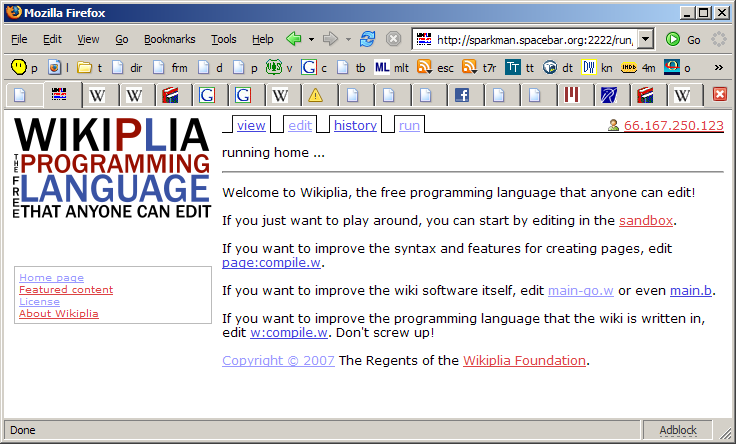
\includegraphics[width=0.92\textwidth]{ss_homepage}
\end{center}
\caption{Screenshot of the Wikiplia home page as of revision
\currentrevision.} \label{fig:sshomepage}
\end{figure*}

\begin{figure*}[t]
\begin{center}
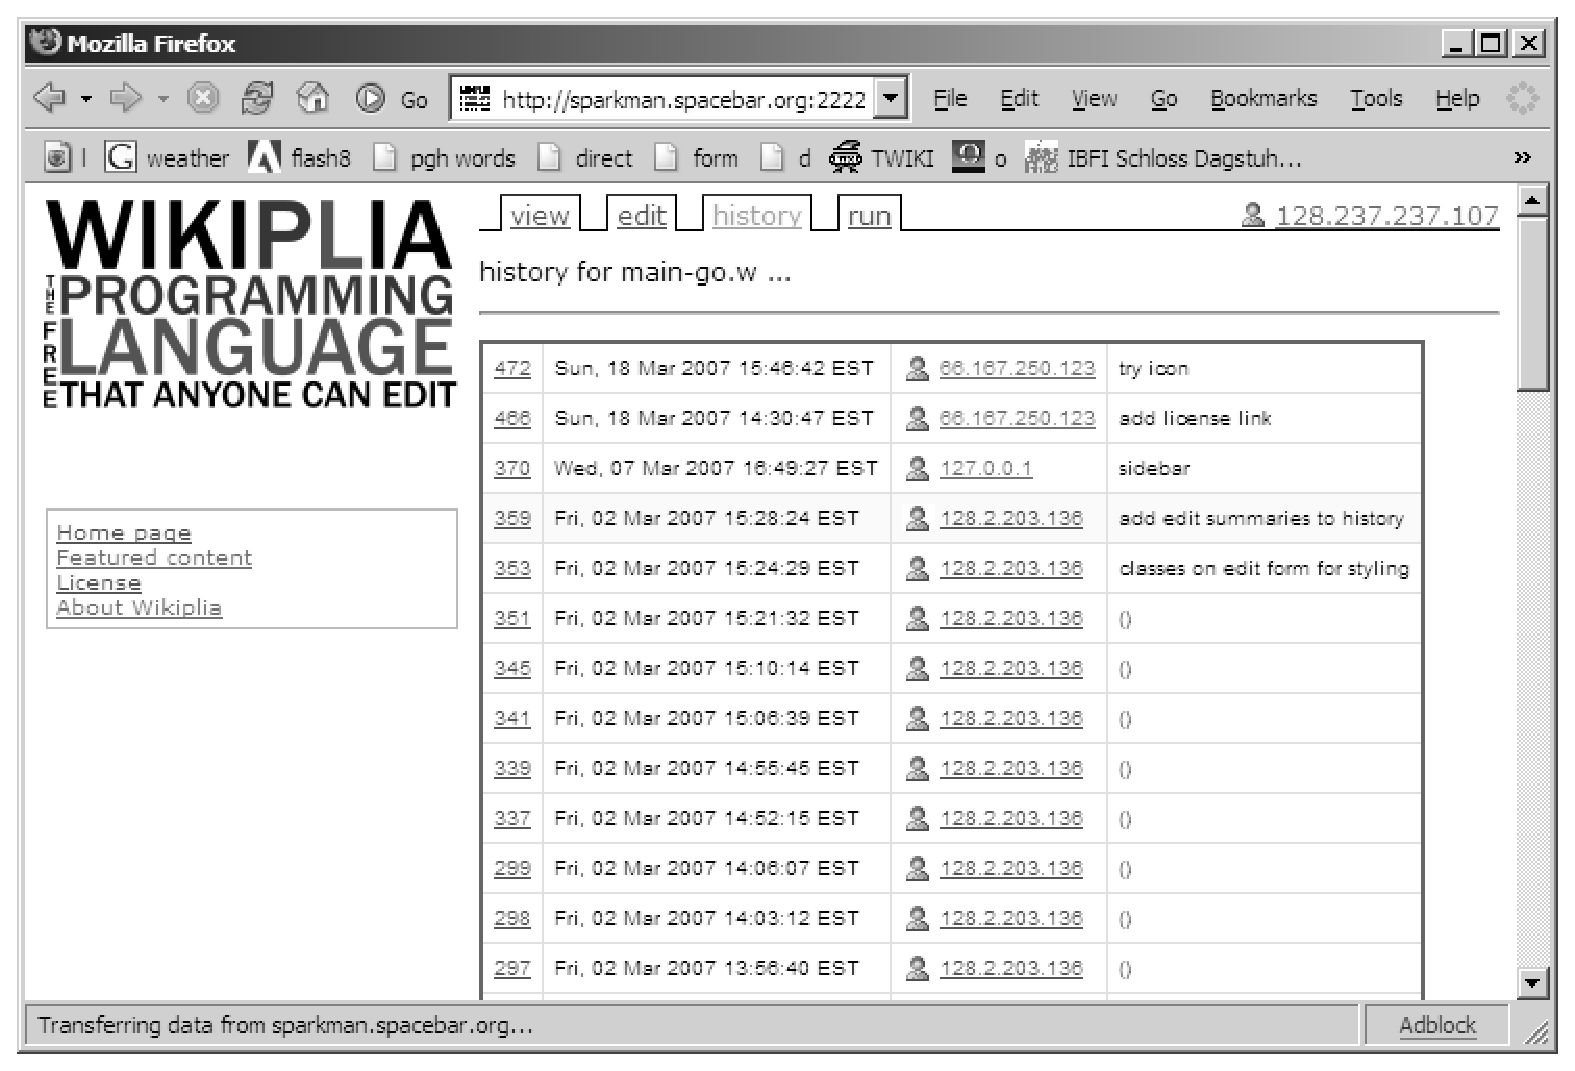
\includegraphics[width=0.92\textwidth]{ss_history}
\end{center}
\caption{Screenshot of the history information for {\tt main-go.w}.
} \label{fig:sshistory}
\end{figure*}

\section{Revision \currentrevision} \label{sec:current}

As of writing, Wikiplia is at revision~\currentrevision, and has
a number of features implemented.

\subsection{Interface}

The editing interface implemented has been enhanced greatly;
Figure~\ref{fig:sshomepage} shows a screenshot of the main page. The
various views of a key are shown with a series of tabs at the top of
each page. Each user has a home page named after his IP
address,\z\wcite{IP address} which he can use to catalogue his
interests. Various warnings help the user, for example, if he tries to
edit a page that was generated by compiling some source code, a
warning message suggests that he may wish to edit the source code
instead. An ornate logo in SVG\wcite{Scalable Vector Graphics} adorns
the page, and a sidebar provides quick access to the site's features.
The logo and graphics for the site are stored in the repository; the
new {\tt raw} and {\tt typed} actions allow access to these resources
over HTTP so that they may be freely modified.\z\footnote{Because
Wikiplia is dogmatically forward-looking, the graphics require SVG
support in the browser and support for the {\tt data:} URL format, a
combination only found in the newest versions of the Mozilla Firefox.
Wikiplia is compatible with incompatible browsers, however, simply
displaying a crapified version of each page.} At revision 228 support
for metadata was added for each page; a {\tt history} tab now shows
the date, revision number, IP address, and edit summary for each
change to a key (Figure~\ref{fig:sshistory}).

% XXX main emergency revert

\subsection{Wikiplia language {\tt w}}

Writing XESP documents by hand is very tedious, so one of the first
orders of business was to develop a compiler for a new language, {\tt
w}, which can be extended with convenient features. The first version
of this language, created in revision 22, was written in XESP. It
automatically quoted the appropriate arguments to the {\sf let}, {\sf
it}, {\sf lambda}, {\sf xcase} primitives. In revision 361, the
compiler was ported to the language {\tt w} as {\tt w:compile.w}, then
compiled with the existing {\tt b}-compiled version of {\tt
w:compile.b}, then recompiled with itself until reaching a fixed
point.\z\wcite{Fixed point (mathematics)} After that, more features
were added: a multi-argument function construct {\tt fn}; a
list-deconstructing binding construct {\tt lets}; simple support for
separately-compiled libraries\wcite{Library (computing)} via {\tt
include}; support for mutually-recursive\wcite{Recursion (computer
science)} bundles of functions via {\tt fun};\footnote{Prior to
this, recursion had to be encoded directly by passing an initial
``self'' argument to each function.} and the {\tt cond} keyword for
series of chained ``if\ldots else'' conditionals. At each stage, the
feature is implemented using the current version of {\tt w}, and then
{\tt w:compile.w} is rewritten to use that convenient extension, and
then recompiled until reaching a fixed point.

\subsection{Wikiplia language {\tt page}}

Wikiplia is not just a programming language; it needs facilities for
editing pages that are human readable as well. This can be used to
edit documentation for programming languages, to modify the home page
to tout new developments, to modify the software license
(Section~\ref{sec:license}) or to deface other user's personal pages.
For this we provide a Wiki-like\wcite{Wiki} syntax that allows for the
authorship of such pages and easy linking between them. Like other
Wikis, a link to a page that does not exist is colored red, to alert
the user to the opportunity to stake out cyberspace real estate. This
syntax is compiled to XESP documents via the {\tt page} language; the
resulting documents are active in the sense that they check the status
of linked pages to report the correct color on every page load.

\section{TIA Public License} \label{sec:license}

In this section we reproduce the Total Information Awareness Public
License. Commentary is given via footnotes\wcite{footnote} into parts
of the license.

{\tt \parindent 0pt \parskip 10pt
\verb+     +TIA PUBLIC LICENSE \\
\verb+   +Revision 468, March 2007

BEGIN INVINCIBLE SECTION 1

This software is Copyright \copyright\ 2007{\large \rm--}$\infty$ The
Regents of the Wikiplia Foundation. Permission is not granted to
reproduce this software or license except by the terms explicitly
enumerated below.

I. Invincible Sections

This license contains certain invincible sections, denoted by the text
``BEGIN INVINCIBLE SECTION <n>'' and ``END INVINCIBLE SECTION <n>''.
Such sections may not be modified under any circumstances. 

END INVINCIBLE SECTION 1\footnote{Invincible sections exist in order
to ensure the sanctity of the license. We first establish that
invincible sections will appear and that they are inviolable; this
itself is done in an invincible section. Invincible sections cause a
limited loss of liberty, but this is the cost of freedom.}

BEGIN INVINCIBLE SECTION 2

II. Version Identification and Invalid Licenses

This license must identify itself in the header as Revision <n> for
some number <n>, which must be the same as the revision number in the
Wikiplia repository for the key ``TPL'' in which the license text is
stored. If this is not the case, then this version of the license is
considered Invalid and Void.

Permission is not granted to distribute the software or license using
any Invalid version of the license.

END INVINCIBLE SECTION 2\footnote{This invincible section establishes
a connection between license versions and the actual contents of the
Wikiplia repository. Note the self-reference: Though this text is in
an invincible section and never changes, the referent of ``this
license'' does change as the rest of the license is modified. Because
Wikiplia assigns version numbers monotonically, this ensures that the
next invincible section is able to guarantee that freedom is
monotonic. In the case of an invalid license, no permissions
whatsoever are granted, so the licensee {\em must} use a prior valid
version of the license. The initial version of the license is valid.}

BEGIN INVINCIBLE SECTION 3

III. Option of License

The licensee has the option to choose any revision of the license
prior to (numerically less than) this version as the licensing
terms for the software and license.

END INVINCIBLE SECTION 3

BEGIN INVINCIBLE SECTION 4

IV. Heredity of License

Any copy or derivative work of this software or license must be
licensed under the TIA Public License.

END INVINCIBLE SECTION 4\footnote{This clause makes the license
``viral'' like the GNU GPL, so that freedom is preserved in all
descendants of the software.}

BEGIN INVINCIBLE SECTION 5

V. Completeness of Copy

This software and license may only be copied in their entirety,
including the entire revision history.

END INVINCIBLE SECTION 5\footnote{This section is the centerpiece of
Wikiplia; it guarantees that the ``source code'' to any software or
programming language derived from Wikiplia is free from the loopholes
described in Section~\ref{sec:bootstrap} and so maximizes
Freedom~\ftinker. Note that this does not limit the way that the
software can be modified; the programmer might begin by blanking all
of the keys he doesn't care about---as long as he preserves the fact
that there was {\em once} something there.}

VI. Freedom to edit

Permission is hereby granted to edit this license.\footnote{The only
non-invincible provision of the original license allows the reader to
add provisions that he desires to the license. This guarantees
Freedom~\ffree, the freedom to redefine freedom.
%
Note that even if a freedom-hater removes this provision from the
license, the invincible sections above ensure that the freedom to edit
the license is preserved for all time.}

}

\bigskip
This license is bootstrapping in the sense that it grants only the
minimal permissions necessary, after setting up invariants via the
behavior-limiting invincible sections. In fact, the original version
of the license does not directly permit the licensee to copy the
% double-entendre with VI intentional
software at all; he must first amend the license using {\tt VI} to
give himself this permission.

\section{Conclusion} \label{sec:conc}

We have reached the end of our journey. But the journey is not
complete! We conclude with a discussion of future plans and unrelated
work, and then conclude with another paragraph.

\subsection{Future Work}

Though Wikiplia in its current form is a usable general-purpose
programming language, work remains to be done for it to reach its full
potential. For one, it needs a vibrant community of contentious and
hubristic editors hiding behind anonymous IP addresses boldly
asserting half-baked syntactic extensions or enforcing superficial
style preferences, gritting their teeth while typing and clicking
white knuckled in a kind of road rage\wcite{List of rages} created by
the dehumanizing semantic markup by which they are forced to
communicate.

% XXX: supporting users with revision #s?

We also seek to improve the languages. The language {\tt w} needs many
more features to speed development: the parenthesis-based XESP syntax
should eventually be replaced by a pleasant concrete syntax, if we can
get around to it before too much code is written in XESP. A type
system\wcite{Type system} is not planned, because type systems
restrict Freedom~\fexpression, the freedom of expression. However, we
should seek to make Wikiplia as multi-paradigm as possible (again,
freedom from discrimination on the basis of paradigm\wcite{paradigm}
orientation), supporting OOPs-oriented
programming,\z\wcite{Object-oriented programming} aspect-oriented
programming,\z\wcite{Aspect-oriented programming} duck-oriented
typing,\z\wcite{Duck typing} orientation-oriented
orienteering,\z\wcite{Orienteering} Orient-oriented
programming,\z\wcite{The Orient} etc.

The {\tt page} language needs extensions for developing human-readable
web pages, mostly for the purpose of creating jazzy graphics and boxes
that distract from or directly call attention to obvious problems with
the pages without actually addressing those problems.

\subsection{Unrelated Work}

All popular modern languages are defined via a definitional
interpreter\wcite{JavaScript}$^,$\wcite{Objective
Caml}$^,$\wcite{Perl} with accompanying O'Reilly ``animal''
book.\z\wcite{O'Reilly Media} The work on Wikiplia is unrelated: We
have no animal mascot\wcite{ORLY owl} and the languages are described
by a tower of source-to-source translations on top of a universally
parseable semantic document in XML\wciteshort{Category:ML programming
language family} form.

The author doesn't think\wcite{Thought} much of
musicals,\z\wcite{Musical theatre} to be perfectly\wcite{Thomas
Aquinas} honest,\z\wcite{Honesty} so those are basically\wcite{BASIC}
a no-go. He also feels that the metric system\wcite{Metric system} but
paradoxically\wcite{Pardadox} also time zones\wcite{Time zone} are
pretty overrated. Ketchup\wcite{Ketchup} on eggs\wcite{Egg (food)} is
gross,\z\wcite{Gross} but not quite as gross as foie gras\wcite{Foie
gras}, which more or less has the word\wcite{Word} ``gross'' in its
name\wcite{Name} so duh.\z\wcite{Duh}

\subsection{Another Paragraph}

We have described Wikiplia, the free programming language that anyone
can edit. Unlike other programming languages, it is designed to
support a variety of freedoms (\ftinker, \fexpression, \fbeer, \fusa,
\ffree, \ftobe) and is explicitly scalable to new freedoms. The system
is implemented in a minimal bootstrapping core, and then built up to
a featured system using its own faculties for extension. XXX more...

\bigskip
$${\tt \wikipliaurl}$$


\end{document}